\documentclass[11pt,a4paper]{article}

\usepackage[
    a4paper,
    left=15mm,
    right=15mm,
    top=30mm,
    bottom=25mm,
    headheight=25mm
]{geometry}
\usepackage{graphicx}
\usepackage{polski}
\usepackage[utf8]{inputenc}
\usepackage{enumerate}
\usepackage{comment}
\usepackage{fancyhdr}
\usepackage{hyperref}
\usepackage{indentfirst}
\usepackage{multirow}
\usepackage{multicol}
\usepackage{float}
\usepackage{amsmath}
\usepackage{fancyhdr}
\usepackage{wrapfig}
\usepackage{layout}
\usepackage{textcomp}
\usepackage[center]{caption}
\usepackage{subcaption}
\usepackage{siunitx}

\sisetup{output-exponent-marker=\ensuremath{\mathrm{e}}}

\renewcommand{\baselinestretch}{1.18}
\renewcommand\thesubfigure{\roman{subfigure}}

\pagestyle{fancy}
\fancyhead[L]{
    
\includegraphics[scale=0.16]{../agh_logo_text_asym.jpg}
}
\fancyhead[R]{
    Lab 2 - Otoczka wypukła | Łukasz Dragon 28.10.2024
}

\begin{document}
\section{Wstęp}
Celem ćwiczenia była implementacja i porównanie 
algorytmów Grahama i Jarvisa wyznaczających otoczkę wypukłą 
na płaszczyźnie oraz wizualizacja otoczek znalezionych
dla wybranych zbiorów punktów.

\subsection{Wstęp teoretyczny}
Otoczkę wypukłą podzbioru punktów definiujemy 
jako najmniejszy (pod względem inkluzji) zbiór wypukły
zawierający ten podzbiór. Zbiór wypukły natomiast to
zbiór, który dla każdej pary punktów w nim zawartych, 
zawiera także odcinek je łączący

W tym ćwiczeniu skupiliśmy się na dwóch algorytmach
wyznaczania otoczki: Grahama i Jarvisa, a dokładniej
ich implementacji dla punktów na płaszczyźnie.

\subsubsection{Algorytm Grahama}
Użyta implementacja algorytmu przebiega następująco:
\begin{enumerate}
    \item \textbf{Znalezienie punktu startowego:}
    Algorytm znajduje punkt $P_0$ o najmniejszej współrzędnej $y$, jeżeli
    jest takich kilka, wybierany jest ten o najmniejszej współrzędnej $x$.
    \item \textbf{Sortowanie względem kąta:}
    Punkty sortowane są rosnąco względem kąta jaki tworzą z punktem $P_0$
    i osią $OX$. Jest to robione przy użyciu funkcji \verb|orient(|$P_0$\verb|, b, c)|,
    która dla danej uporządkowanej trójki punktów zwraca jej "skrętność": 
    zgodnie lub wbrew ruchowi wskazówek zegara. 
    Skrętność zgodna z ruchem wskazówek zegara oznacza, że punkt \verb|b|
    znajdzie się przed punktem \verb|a|, a odwrotna skrętność ustawi
    punkt \verb|a| przed \verb|b|. Po sortowaniu, punkty 
    tworzące ten sam kąt są usuwane, poza tym najbardziej odległym od punktu $P_0$.
    Funkcję \verb|orient| zaimplementowałem metodą wyznacznika 
    macierzy $3\times3$, a samo sortowanie zaimplementowałem algorytmem
    \textit{QuickSort}.
    \item \textbf{Tworzenie otoczki:}
    Tworzony jest stos $S$, który zawierać będzie kandydatów na
    punkty wynikowej otoczki. Następnie sprawdzamy po kolei każdy
    punkt z posortowanej listy, wykonując następujące czynności:
    \begin{itemize}
        \item Jeżeli dwa górne punkty z $S$ tworzą z rozważanym
        punktem skręt wbrew ruchowi wskazówek zegara, to powinien
        należeć do otoczki, więc dodajemy go na górę stosu.
        \item Jeżeli punkty tworzą odwrotny skręt, bądź są kolinearne
        to usuwamy górny punkt z $S$ i powtarzamy sprawdzenie skrętności,
        aż będzie odpowiednia.
    \end{itemize}
    \item \textbf{Wynik:} Wynikiem są punkty w $S$ wraz z $P_0$.
\end{enumerate}

\begin{tabular}{l|l|}
    Złożoność obliczeniowa: & $O(nlogn)$ \\
    Złożoność pamięciowa: & $O(n)$ \\
\end{tabular}
\footnotesize gdzie $n$ oznacza liczbę punktów. \normalsize

\pagebreak

\subsubsection{Algorytm Jarvisa}
Niech $Q$ oznacza dany zbiór punktów.

Użyta implementacja algorytmu przebiega następująco:
\begin{enumerate}
    \item \textbf{Znalezienie punktu startowego:}
    Algorytm znajduje punkt $P_0$ o najmniejszej współrzędnej $y$, jeżeli
    jest takich kilka, wybierany jest ten o najmniejszej współrzędnej $x$.
    \item \textbf{Iteracyjne szukanie punktów do otoczki:}
    Zaczynając od punktu $P_0$ szukamy kolejnych punktów $P_i$
    należących do otoczki. Robimy to kolejno szukając punktu $P_i$,
    dla którego:

    $\forall q\in Q \quad \text{układ} \quad P_{i - 1}, P_i, q \quad
    \text{tworzy skręt wbrew ruchowi wskazówek zegara.}$
    
    \centering
    \footnotesize(korzystając z funkcji \verb|orient|).

    \raggedright
    \normalsize
    Dla punktów współliniowych wybieramy ten, 
    który jest najbardziej oddalony od $P_i$.
    \item \textbf{Wynik:}
    Algorytm kończy działanie kiedy $P_i = P_0$. Zbiór punktów 
    zawierający wszystkie znalezione punkty $P_i$ jest wynikiem.
\end{enumerate}

\begin{tabular}{l|l|l}
    Złożoność obliczeniowa: & $O(nh)$ & \footnotesize gdzie $n$ oznacza liczbę wszytkich punktów\\
    Złożoność pamięciowa: & $O(h)$ &  \footnotesize i $h$ oznacza liczbę punktów w otoczce.\\
\end{tabular}

\subsection{Specyfikacja narzędzi i sprzętu}
Wszystkie potrzebne obliczenia zostały wykonane przy użyciu interpretera języka Python wersji 3.12.
Ponadto, w celu wygenerowania zbiorów punktów użyłem biblioteki numpy. Wykresy i wizualizacja wyników została przygotowana za pomocą narzędzia
przygotowanego przez koło naukowe Bit. Kod znajduje się w załączonym pliku.
Przedstawione wyniki zostały wygenerowane na komputerze z systemem operacyjnym Debian 12 i 
procesorem AMD Ryzen 5 3600 3.6GHz.

\pagebreak

\section{Realizacja obliczeń}
Obliczenia rozpocząłem od przygotowania czterech zbiorów losowych punktów,
zwizualizowanych na Rysunku 1:

\begin{figure}[H]
    \centering
    \begin{subfigure}[b]{0.46\textwidth}
        \centering
        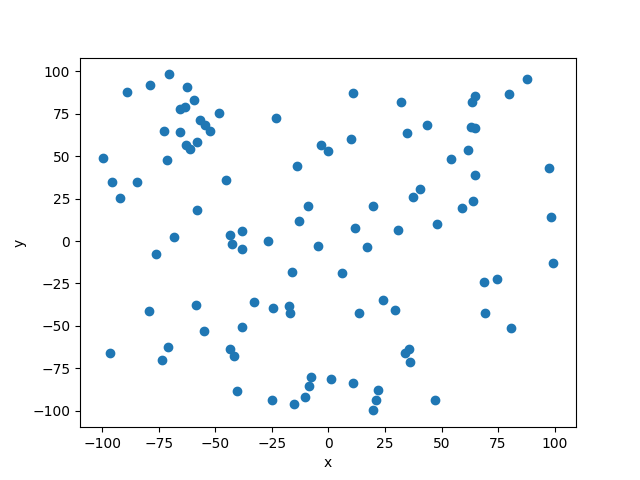
\includegraphics[scale=0.5]{res/points_a.png}
        \caption{
            Zbiór A 
            \\ 
            \footnotesize$100$ punktów o współrzędnych
            \\
            z przedziału $[-100, 100]$.
        }
    \end{subfigure}
    \begin{subfigure}[b]{0.46\textwidth}
        \centering
        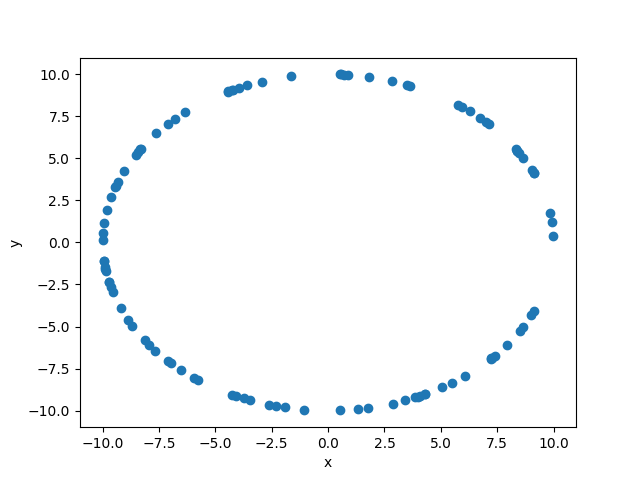
\includegraphics[scale=0.5]{res/points_b.png}
        \caption{
            Zbiór B
            \\
            \footnotesize$100$ punktów na okręgu: $x^2 + y^2 = 100$.
            \\
            ~
        }
    \end{subfigure}
    \begin{subfigure}[b]{0.46\textwidth}
        \centering
        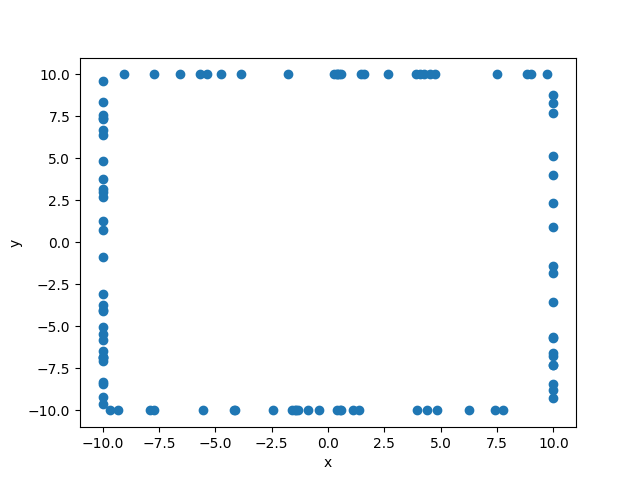
\includegraphics[scale=0.5]{res/points_c.png}
        \caption{
            Zbiór C
            \\
            \footnotesize$100$ punktów na bokach prostokąta
            o wierzchołkach:
            \\
            (-10, 10), (-10, -10), (10, -10), (10, 10)
            \\
            ~
        }
    \end{subfigure}
    \begin{subfigure}[b]{0.46\textwidth}
        \centering
        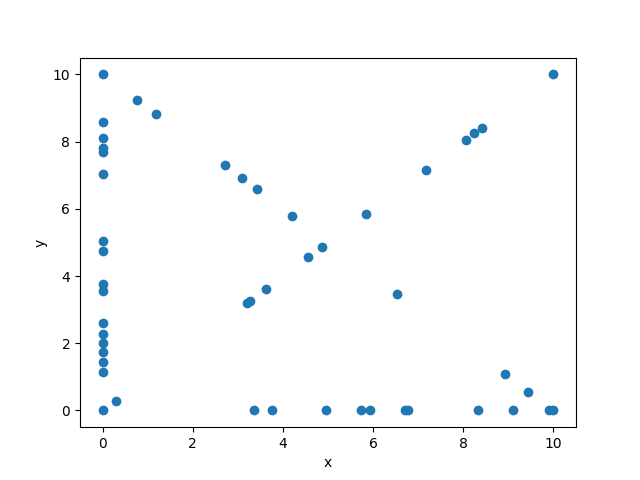
\includegraphics[scale=0.5]{res/points_d.png}
        \caption{
            Zbiór D
            \\
            \footnotesize Wierzchołki kwadratu: (0,0), (10, 0), (10, 10), (0, 10)
            \\
            oraz 25 punktów na jego bokach leżących na osiach
            i 20 punktów na jego przękątnych.
        }
    \end{subfigure}
    \caption{Wygenerowane zbiory}
\end{figure}

Następnie wyznaczyłem otoczki wypukłe dla każdego zbioru oboma
algorytmami, tworząc animacje wizualizujące działanie każdego z nich
(punkty należące do otoczki wypisywane są w załączonym kodzie, 
wybrane animacje załączone są razem ze sprawozdaniem).
Ostatecznie przygotowałem liczniejsze, lecz stworzone analogicznie zbiory
w celu porównania czasu wykonania algorytmów dla każdego z nich.
W kolejnej sekcji przedstawiam wizualizacje i wyniki moich obliczeń.

\section{Wyniki}

\subsection{Wizualizacja otoczek wypukłych}
Rysunek 2 zawiera zwizualizowane otoczki wypukłe dla 
zbiorów A, B, C i D. Punkty zawarte w otoczce zaznaczone
są kolorem czerwonym, a krawędzie otoczki pomarańczowym.

\begin{figure}[H]
    \centering
    \begin{subfigure}[b]{0.46\textwidth}
        \centering
        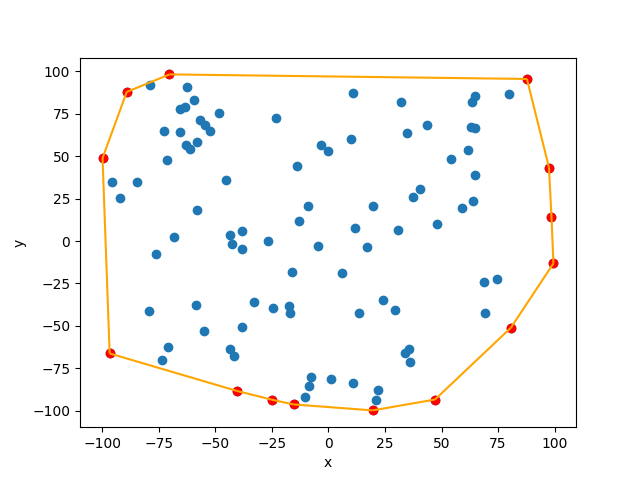
\includegraphics[scale=0.5]{res/graham_a.png}
        \caption{
            Zbiór A 
        }
    \end{subfigure}
    \begin{subfigure}[b]{0.46\textwidth}
        \centering
        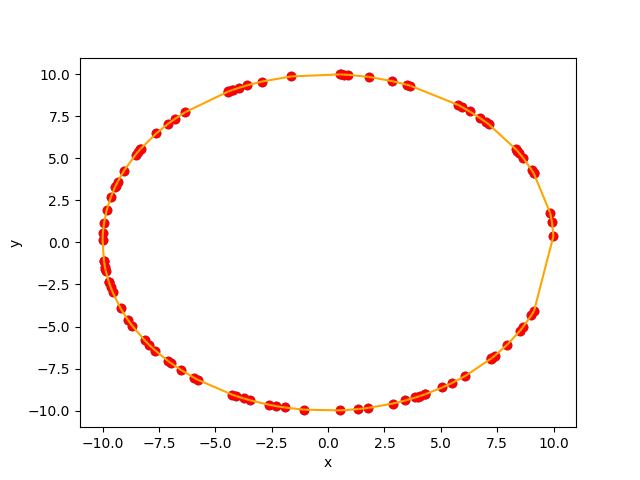
\includegraphics[scale=0.5]{res/graham_b.png}
        \caption{
            Zbiór B
        }
    \end{subfigure}
    \begin{subfigure}[b]{0.46\textwidth}
        \centering
        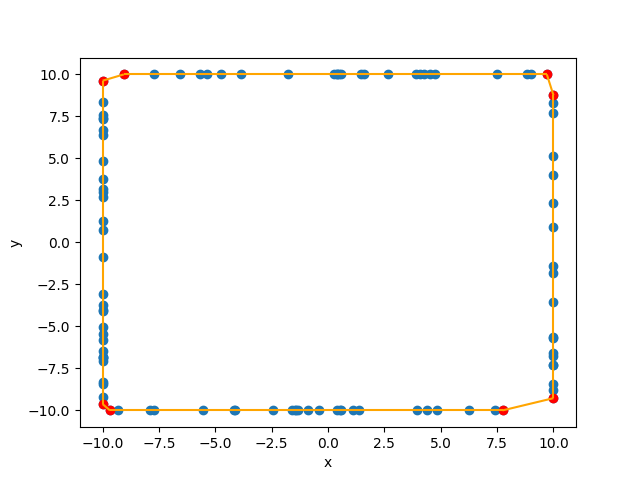
\includegraphics[scale=0.5]{res/graham_c.png}
        \caption{
            Zbiór C
        }
    \end{subfigure}
    \begin{subfigure}[b]{0.46\textwidth}
        \centering
        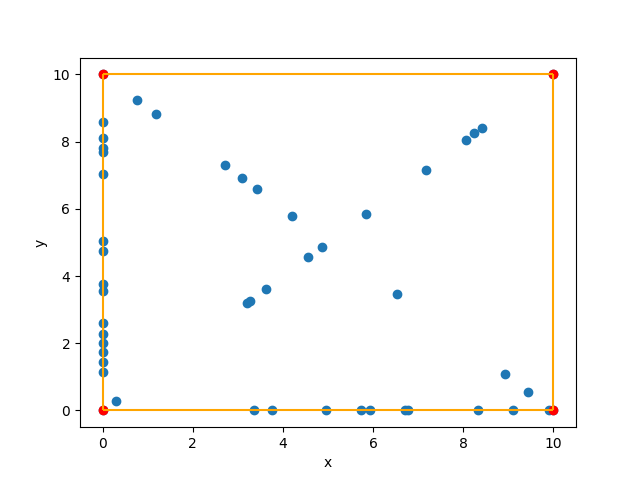
\includegraphics[scale=0.5]{res/graham_d.png}
        \caption{
            Zbiór D
        }
    \end{subfigure}
    \caption{Wyznaczone otoczki}
\end{figure}

Implementacje obu algorytmów zwracały te same wyniki dla sprawdzanych
zbiorów. Lista punktów należących do otoczek wygenerowanych przez oba 
algorytmy wypisywana jest w załączonym kodzie.

\pagebreak

\subsection{Porównanie algorytmów}
Algorytmy porównywałem na następująco zmodyfikowanych
zbiorach A, B, C i D:
\begin{itemize}
    \item \textbf{Zbiór A:}
    $n$ punktów o współrzędnych
    z przedziału $[-10000, 10000]$.
    \item \textbf{Zbiór B:} 
    $n$ punktów na okręgu: $x^2 + y^2 = 10000$.
    \item \textbf{Zbiór C:}
    $n$ punktów na bokach prostokąta
    o wierzchołkach:\\
    (-100, 100), (-100, -100), (100, -100), (100, 100)
    \item \textbf{Zbiór D:}
    Wierzchołki kwadratu: \\
    (0,0), (10, 0), (10, 10), (0, 10)\\
    oraz $\lfloor \frac{n}{2} \rfloor - 5$ punktów na jego bokach leżących na osiach
    i $\lfloor \frac{n}{2} \rfloor + 5$ punktów na jego przękątnych.
\end{itemize}

gdzie $n\in\{10, 50, 100, 1000, 10000\}$.

Tabele 1, 2, 3, 4 zawierają czasy wykonania algorytmów
Grahama (\verb|graham_algorithm|) \\
i Jarvisa (\verb|jarvis_algorithm|)
w sekundach zaokrąglone do $1\si{\micro s}$ dla poszczególnych
zbiorów i wartości $n$. Rysunki 3, 4, 5, 6 zawierają wykresy zależności
zawartych w tabelach. Należy zwrócić uwagę na różne skale osi pionowych 
na wykresach.

\subsubsection{Zbiór A}
\begin{table}[H]
    \centering
    \begin{tabular}{|l|r|r|r|r|r|}
    \hline
        $n$ & 10 & 50 & 100 & 1000 & 10000 \\ \hline
        \verb|graham_algorithm| & 0.000210s & 0.001478s & 0.002029s & 0.027338s & 0.313523s \\ \hline
        \verb|jarvis_algorithm| & 0.000188s & 0.001711s & 0.003523s & 0.074435s & 0.815001s \\ \hline
    \end{tabular}
    \caption{Porównanie czasu wykonania algorytymów dla zbiorów typu A}
\end{table}

Czasy wykonania obu algorytmów w tym zbiorze są zbliżone do siebie,
lecz algorytm Jarvisa staje się znacząco wolniejszy od algorytmu Grahama
dla większych wartości $n$. Punkty w zbiorze A są wygenerowane losowo
wewnątrz prostokąta, co oznacza, że większość z nich nie będzie należeć do 
otoczki. Dzięki temu, czasy wykonania algorytmu Jarvisa nie odstają tak 
znacząco od czasów algorytmu Grahama, jak chociażby w zbiorze B. 
Mimo wszystko, wraz z większą liczbą punktów, zwiększa się także liczba
punktów na otoczce, co znacząco pogarsza złożoność obliczeniową 
algorytmu Jarvisa w porównaniu do złożoności algorytmu Grahama,
która pozostaje ta sama.

\begin{figure}[H]
    \centering
    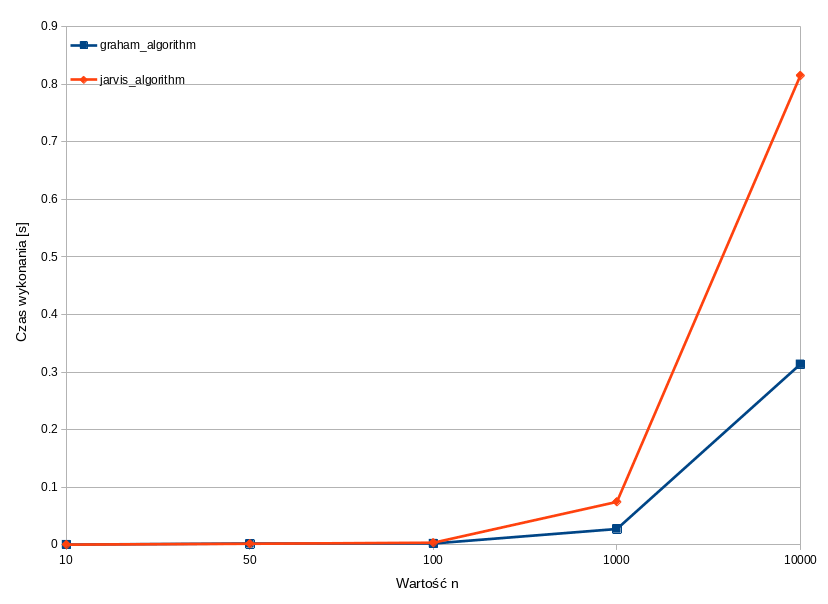
\includegraphics[scale=0.6]{res/wykres_a.png}
    \caption{Wykres zależności czasu wykonania 
    od $n$ dla obu algorytmów (Zbiór A).}
\end{figure}

\subsubsection{Zbiór B}
\begin{table}[H]
    \centering
    \begin{tabular}{|l|r|r|r|r|r|}
    \hline
        $n$ & 10 & 50 & 100 & 1000 & 10000 \\ \hline
        \verb|graham_algorithm| & 0,000085s & 0.000601s & 0.001589s & 0.020120s & 0.275786s \\ \hline
        \verb|jarvis_algorithm| & 0.000230s & 0.004347s & 0.017882s & 1.774898s & 175.497906s \\ \hline
    \end{tabular}
    \caption{Porównanie czasu wykonania algorytymów dla zbiorów typu B}
\end{table}

Zbiór B wyraźnie pokazuje różnice między obiema metodami; czasy
wykonania algorytmu Jarvisa są znacząco większe dla każdych wartości $n$. 
Wynika to z faktu, iż do zbioru należą tylko punkty na okręgu, 
co oznacza, że każdy z nich zawarty jest w otoczce. Dla $n$ punktów 
złożoność obliczeniowa algorytmu Jarvisa jest wtedy rzędu $O(n^2)$.
Dla największej sprawdzonej wartości $n$ widzimy przez to niemal 600-krotne
pogorszenie czasu względem algorytmu Grahama.

\begin{figure}[H]
    \centering
    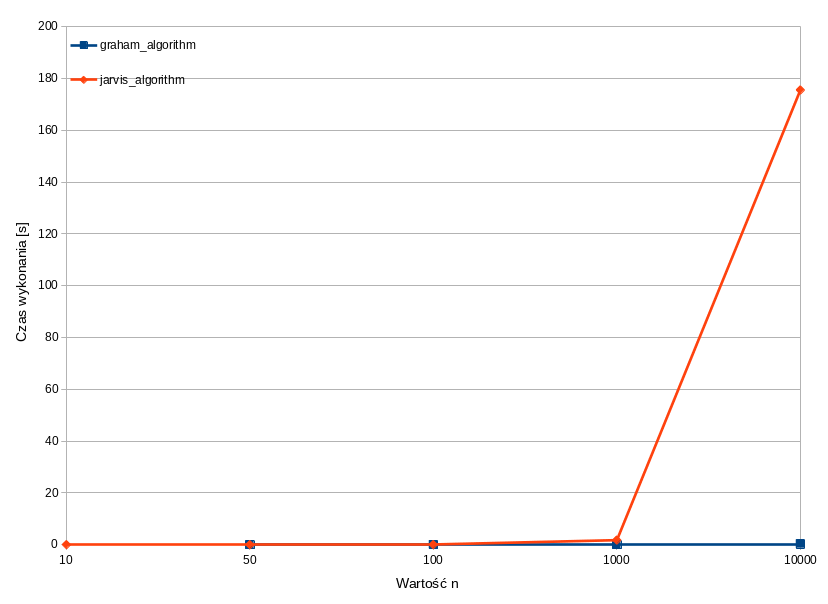
\includegraphics[scale=0.6]{res/wykres_b.png}
    \caption{Wykres zależności czasu wykonania 
    od $n$ dla obu algorytmów (Zbiór B).}
\end{figure}

\subsubsection{Zbiór C}
\begin{table}[H]
    \centering
    \begin{tabular}{|l|r|r|r|r|r|}
    \hline
        $n$ & 10 & 50 & 100 & 1000 & 10000 \\ \hline
        \verb|graham_algorithm| & 0.000062s & 0.000379s & 0.000920s & 0.016762s & 0.522928s \\ \hline
        \verb|jarvis_algorithm| & 0.000110s & 0.000728s & 0.001513s & 0.016282s & 0.156463s \\ \hline
    \end{tabular}
    \caption{Porównanie czasu wykonania algorytymów dla zbiorów typu C}
\end{table}

W tym zbiorze po raz pierwszy widzimy przewagę algorytmu Jarvisa.
Wynika ona z faktu, iż w najgorszym przypadku otoczka losowych punktów
na obwodzie prostokątu będzie zawierać tylko 8 punktów. Dzięki temu,
możemy uznać złożoność obliczeniową metody Jarvisa jako liniową.
Dla małych wartości $n$ algorytm Grahama nadal wykonuje się szybciej,
lecz wraz ze zwiększeniem liczby punktów, czasy wykonania algorytmu Jarvisa
rosną w mniejszym tempie, niż te odpowiadające metodzie Grahama.

\begin{figure}[H]
    \centering
    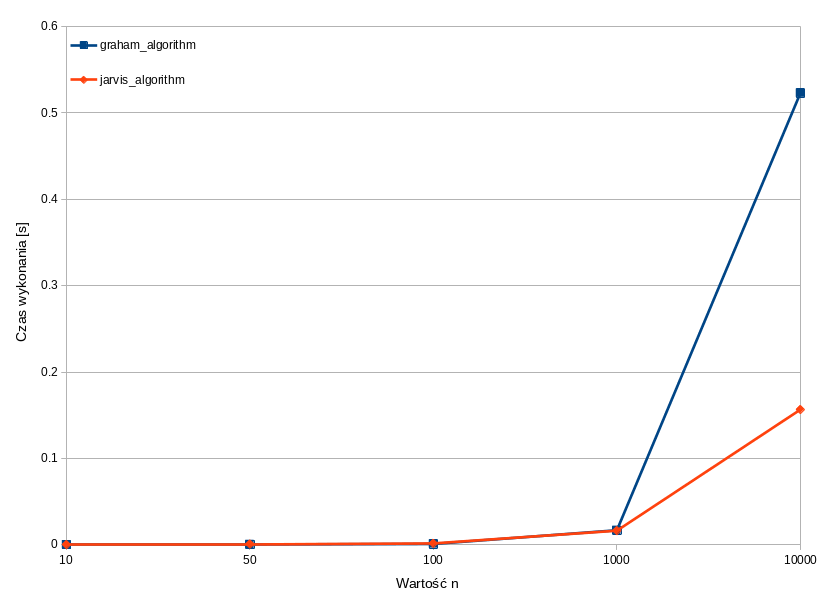
\includegraphics[scale=0.6]{res/wykres_c.png}
    \caption{Wykres zależności czasu wykonania 
    od $n$ dla obu algorytmów (Zbiór C).}
\end{figure}

\subsubsection{Zbiór D}
\begin{table}[H]
    \centering
    \begin{tabular}{|l|r|r|r|r|r|}
    \hline
        $n$ & 10 & 50 & 100 & 1000 & 10000 \\ \hline
        \verb|graham_algorithm| & 0.000112s & 0.000585s & 0.001395s & 0.087795s & 7.754411s \\ \hline
        \verb|jarvis_algorithm| & 0.000181s & 0.000608s & 0.001176s & 0.016209s & 0.093529s \\ \hline
    \end{tabular}
    \caption{Porównanie czasu wykonania algorytymów dla zbiorów typu D}
\end{table}

Wyniki dla zbioru D pokazują przewagę czasową dla algorytmu
Jarvisa, która początkowo nieznaczna, rośnie dla większych wartości $n$.
Podobnie jak w \\zbiorze C, wynika to z faktu iż liczba punktów
w otoczce jest bardzo mała (w tym zbiorze jest zawsze równa 4), co
umożliwia algorytmowi Jarvisa na wykonanie się w czasie liniowym.
Różnicą miedzy tymi zbiorami jest jednak wystąpienie punktów na 
obu przekątnych, szczególnie tej przechodzącej przez punkt $(10,0)$, 
których algorytm Grahama nie jest w stanie usunąć w kroku 2 opisanym
w sekcji 1.1.1. Najlepiej ten fakt pokazuje animacja załączona
ze sprawozdaniem.

Należy jednak zauważyć, że sortowanie punktów w algorytmie Grahama
zostało zaimplementowane algorytmem \textit{QuickSort}, co najprawdopodobniej
wpłynęło na znacząco gorszy czas dla $n = 1000$, ponieważ algorytm ten w 
najgorszym wypadku ma złożoność $O(n^2)$.

\begin{figure}[H]
    \centering
    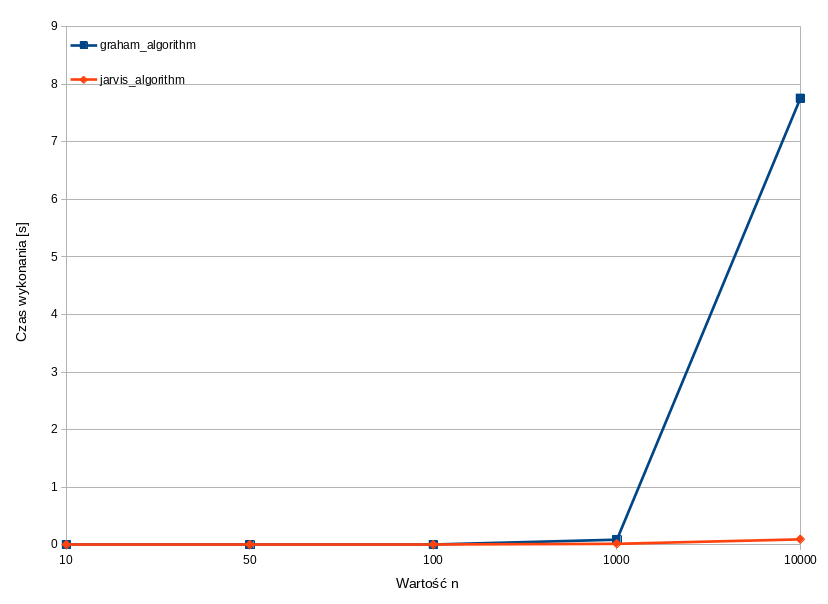
\includegraphics[scale=0.6]{res/wykres_d.png}
    \caption{Wykres zależności czasu wykonania 
    od $n$ dla obu algorytmów (Zbiór D).}
\end{figure}

\section{Podsumowanie}
Przyrównując czasy wykonania obu algorytmów dla różnych zbiorów
możemy jasno zobaczyć różnicę między nimi. Mimo tego, iż algorytm Grahama
wykonywał się średnio szybciej, to algorytm Jarvisa okazał się szybszy
dla zbiorów C i D. Jest tak, ponieważ otoczka tych zbiorów zawierała
w sobie małą liczbę punktów, przez co liczba wykonywanych operacji
w algorytmie Jarvisa rosła niemal liniowo. Najlepiej pokazał to zbiór D,
w którym metoda Jarvisa okazała się nawet dużo szybsza od Grahama.

W zbiorze B zobaczyć można znaczącą przewagę algorytmu Grahama, który
dla wartości $n = 10000$ wykonywał się niemal 90 razy szybciej. 
Wynika to z faktu, iż każdy punkt w tym zbiorze należy do otoczki, co
oznacza, że złożoność obliczeniowa algorytmu Jarvisa jest rzędu $O(n^2)$

Ostatecznie możemy dojść do wniosku, iż algorytm Grahama jest szybszy
w większej liczbie przypadków (zależne jest to też oczywiście od implementacji
algorytmu sortowania), lecz w przypadkach, w których otoczka wypukła zawiera
mało lub nawet stałą liczbę punktów, algorytm Jarvisa jest w stanie osiągnąć
lepszą złożoność obliczeniową od algorytmu Grahama.

\end{document}
